\documentclass[11pt,a4paper]{article}

% Packages
\usepackage[utf8]{inputenc}
\usepackage[margin=1in]{geometry}
\usepackage{amsmath,amssymb,amsfonts}
\usepackage{graphicx}
\usepackage{booktabs}
\usepackage{algorithm}
\usepackage{algpseudocode}
\usepackage{hyperref}
\usepackage{caption}
\usepackage{subcaption}
\usepackage{float}
\usepackage{siunitx}
\usepackage{multirow}
\usepackage{array}
\usepackage{xcolor}
\usepackage{tikz}
\usetikzlibrary{positioning,arrows.meta,shapes.geometric,calc,fit,backgrounds,decorations.pathreplacing}

% Hyperref settings
\hypersetup{
    colorlinks=true,
    linkcolor=blue,
    citecolor=blue,
    urlcolor=blue
}

% Title and authors
\title{\textbf{Physics-Informed Neural Networks for Hemodynamic Prediction in Cerebral Aneurysms: A Sparse Data Learning Approach}}

\author{
    % Add author names here
    \textit{Authors}
}

\date{}

\begin{document}

\maketitle

\begin{abstract}
Predicting hemodynamic parameters within cerebral aneurysms remains a significant challenge in neurovascular medicine, particularly when assessing rupture risk and planning interventions. Whilst traditional computational fluid dynamics (CFD) simulations provide detailed flow information, they demand substantial computational resources and time-consuming mesh generation for patient-specific geometries. We present a physics-informed neural network (PINN) approach that addresses these limitations by learning from sparse CFD data---using only 10\% of available measurements---whilst simultaneously enforcing fundamental physical laws governing blood flow. Our framework integrates the incompressible Navier-Stokes equations with a non-Newtonian Carreau-Yasuda viscosity model to capture the shear-thinning behaviour of blood, implements pulsatile inlet conditions derived from physiological waveforms, and predicts wall shear stress (WSS) patterns across six anatomically distinct aneurysm configurations. Through careful weighting of data-driven and physics-based loss terms, the network achieves coefficient of determination values exceeding 0.85 for velocity components and 0.80 for pressure predictions, despite the significant data sparsity. The model converges within approximately 2,000 training epochs and successfully reproduces complex haemodynamic features, including recirculation zones and WSS distributions crucial for clinical decision-making. Our findings suggest that physics-informed machine learning offers a practical pathway towards rapid, accurate hemodynamic analysis in neurovascular clinics.

\noindent \textbf{Keywords:} Physics-Informed Neural Networks, Cerebral Aneurysms, Haemodynamics, Wall Shear Stress, Navier-Stokes Equations, Sparse Data Learning
\end{abstract}

\section{Introduction}

Cerebral aneurysms represent pathological dilations of intracranial blood vessels, with prevalence estimates ranging between 3--5\% in the general population \cite{ref1}. When these weakened vessel walls rupture, the resulting subarachnoid haemorrhage carries devastating consequences, with mortality rates frequently exceeding 50\% \cite{ref2}. Clinicians therefore face the challenging task of stratifying rupture risk to guide treatment decisions, weighing the benefits of preventive intervention---such as surgical clipping or endovascular coiling---against the inherent procedural risks.

The haemodynamic environment within an aneurysm, characterised particularly by wall shear stress (WSS) patterns, has emerged as a critical determinant of vessel wall stability and rupture propensity \cite{ref3,ref4}. Regions subjected to abnormally low WSS tend to exhibit continued aneurysm growth and heightened rupture risk, whilst areas experiencing elevated WSS may indicate flow impingement sites where the vessel wall experiences concentrated mechanical stress. Over the past two decades, computational fluid dynamics (CFD) has established itself as the principal tool for non-invasive haemodynamic analysis, offering detailed visualisation of three-dimensional flow structures and quantitative assessment of WSS distributions \cite{ref5,ref6}.

Despite its proven utility, CFD analysis confronts several persistent challenges that limit its clinical adoption. High-fidelity simulations demand considerable computational resources, particularly when modelling pulsatile blood flow through the cardiac cycle using Reynolds-Averaged Navier-Stokes (RANS) turbulence formulations. The process of generating suitable computational meshes for patient-specific geometries remains labour-intensive, requiring specialist expertise and often consuming hours of manual refinement to ensure mesh quality. Furthermore, CFD predictions exhibit sensitivity to numerous modelling assumptions---including inlet and outlet boundary conditions, turbulence closure schemes, and arterial wall compliance---which collectively introduce uncertainty into the haemodynamic assessments that clinicians rely upon for treatment planning.

Physics-informed neural networks (PINNs) \cite{raissi2019pinns} present an intriguing alternative paradigm that may address these limitations. Rather than treating governing equations and observational data as separate entities, PINNs embed physical laws directly into the learning process through carefully constructed loss functions that penalise deviations from known conservation principles. This synthesis of data-driven flexibility with physics-based rigour enables the network to interpolate sparse measurements whilst maintaining consistency with fundamental fluid mechanics.

\subsection{Contributions}

This investigation makes several distinct contributions to the application of physics-informed machine learning in vascular haemodynamics. First, we demonstrate that PINNs can achieve clinically relevant accuracy whilst learning from dramatically reduced datasets---specifically, training on only 10\% of available CFD measurements by enforcing conservation laws at randomly sampled collocation points throughout the flow domain. Second, we implement a comprehensive treatment of physiologically realistic boundary conditions, including time-varying pulsatile inlet velocity profiles derived from published cardiac waveforms, zero-pressure outlet conditions, and rigorous enforcement of no-slip constraints at vessel walls through carefully tuned adaptive weighting schemes.

Our framework explicitly accounts for blood's non-Newtonian rheological behaviour through the Carreau-Yasuda viscosity model, recognising that shear-thinning effects become particularly pronounced in the low-velocity recirculation zones characteristic of aneurysm sacs. To assess the generalisability of our approach across diverse anatomical scenarios, we conduct systematic evaluation on six distinct aneurysm configurations, varying both overall size (5~cm versus 6~cm diameter) and morphological features (baseline, asymmetric saccular with downstream or upstream positioning). Finally, our temporal modelling strategy captures haemodynamic variations across the cardiac cycle by training networks to predict flow characteristics during both systolic peak flow and diastolic minimum flow phases, with explicit enforcement of the pulsatile inlet waveform throughout.

The remainder of this paper proceeds as follows. Section~2 positions our work within the broader context of CFD-based aneurysm analysis and emerging machine learning approaches. Section~3 details our methodology, including the problem formulation, network architecture, and physics-informed loss construction. Section~4 describes our experimental framework and the six aneurysm configurations under investigation. Section~5 presents quantitative performance metrics alongside qualitative visualisations of predicted flow fields. Section~6 discusses the implications of our findings for clinical application, addresses current limitations, and outlines promising directions for future development. Section~7 provides concluding remarks.

\section{Related Work}

\subsection{CFD in Aneurysm Hemodynamics}

Computational fluid dynamics has been extensively applied to aneurysm analysis. Cebral et al. \cite{ref7} demonstrated correlations between WSS patterns and aneurysm rupture through large-scale patient studies. Xiang et al. \cite{ref8} developed hemodynamic indices combining WSS, oscillatory shear index (OSI), and flow stability metrics. However, CFD simulations typically require hours to days of computation per patient, limiting real-time clinical application.

\subsection{Machine Learning for Hemodynamics}

Traditional machine learning approaches have been applied to predict hemodynamic quantities from geometric features. Liang et al. \cite{ref9} used support vector machines to classify rupture risk based on morphological parameters. More recently, convolutional neural networks have been employed to predict CFD outcomes from 3D geometries \cite{ref10}, though these methods lack explicit physics encoding and require extensive training datasets.

\subsection{Physics-Informed Neural Networks}

Raissi et al. \cite{raissi2019pinns} introduced PINNs for solving forward and inverse problems in partial differential equations (PDEs). The key innovation is incorporating PDE residuals directly into the loss function, enabling networks to interpolate sparse data while satisfying conservation laws. PINNs have been successfully applied to fluid dynamics \cite{ref11}, heat transfer \cite{ref12}, and material modeling \cite{ref13}.

In cardiovascular applications, Arzani et al. \cite{ref14} applied PINNs to synthetic arterial flow problems, demonstrating superior performance over pure data-driven methods. However, application to complex patient-specific aneurysm geometries with pulsatile flow and non-Newtonian rheology remains unexplored.

\section{Methodology}

We describe a physics-informed neural network (PINN) that approximates steady Reynolds-averaged haemodynamics for two cardiac phases (systolic and diastolic) in aneurysm domains. The formulation couples data-driven fitting at the wall (pressure, WSS) with interior enforcement of the incompressible RANS equations, non-Newtonian Carreau-Yasuda viscosity, and a \emph{learnable} turbulent viscosity field. This section is structured as: problem formulation and governing equations (\S\ref{sec:problem}), non-dimensionalisation and standardisation (\S\ref{sec:nondim}), network architecture (\S\ref{sec:arch}), loss construction and weighting (\S\ref{sec:loss}), and training procedure (\S\ref{sec:training}).

%==============================================================================
\subsection{Problem Formulation and Governing Equations}
\label{sec:problem}
%==============================================================================

We consider incompressible flow in a bounded domain $\Omega \subset \mathbb{R}^3$ (aneurysm lumen). The reference CFD was produced with the SST $k$--$\omega$ transition model and Carreau-Yasuda blood rheology; we therefore pose the \emph{Reynolds-averaged} momentum and continuity equations with an effective viscosity that combines molecular (shear-dependent) and turbulent contributions.

\subsubsection{RANS and Effective Viscosity}

The flow is governed by
\begin{equation}
\nabla \cdot \mathbf{u} = 0 \quad \text{(continuity)}
\label{eq:continuity}
\end{equation}
and
\begin{equation}
\rho \, \mathbf{u} \cdot \nabla \mathbf{u} = -\nabla p + \nabla \cdot \boldsymbol{\tau}_{\text{eff}} \quad \text{(momentum, steady RANS)}
\label{eq:momentum}
\end{equation}
where $\mathbf{u} = (u,v,w)^T$ is the velocity, $p$ is pressure, $\rho = 1060$\,kg/m$^3$, and the deviatoric stress is
\begin{equation}
\boldsymbol{\tau}_{\text{eff}} = \mu_{\text{eff}} \bigl( \nabla\mathbf{u} + (\nabla\mathbf{u})^T \bigr), \qquad \mu_{\text{eff}} = \mu(\dot{\gamma}) + \rho\,\nu_t.
\label{eq:tau_eff}
\end{equation}
Here $\mu(\dot{\gamma})$ is the shear-dependent molecular viscosity (Carreau--Yasuda) and $\nu_t$ is the turbulent kinematic viscosity, which we treat as a \emph{learnable field} $\nu_t(\mathbf{x}; t_{\text{phase}})$ output by a separate network (see \S\ref{sec:arch}). Temporal dependence is captured by training on two discrete phases---systole and diastole---encoded as a scalar $t_{\text{phase}} \in \{0,1\}$; the same networks then approximate the flow at any query point $(\mathbf{x}, t_{\text{phase}})$.

\subsubsection{Non-Newtonian Molecular Viscosity (Carreau--Yasuda)}
\label{sec:carreau}

Blood exhibits shear-thinning: viscosity decreases with increasing shear rate. We use the Carreau--Yasuda model
\begin{equation}
\mu(\dot{\gamma}) = \mu_\infty + (\mu_0 - \mu_\infty) \left[ 1 + (\lambda \dot{\gamma})^a \right]^{(n-1)/a},
\label{eq:carreau}
\end{equation}
with $\mu_\infty = 0.0035$\,Pa\,s, $\mu_0 = 0.16$\,Pa\,s, $\lambda = 8.2$\,s, $n = 0.2128$, $a = 0.64$. The shear rate is $\dot{\gamma} = \sqrt{2\,\mathrm{tr}(\mathbf{D}^2)}$ where $\mathbf{D} = \frac{1}{2}(\nabla\mathbf{u} + (\nabla\mathbf{u})^T)$. In the momentum residual we use $\mu(\dot{\gamma})$ at each collocation point; to avoid prohibitively expensive third derivatives, we adopt a \emph{quasi-steady} approximation: $\mu_{\text{mol}}$ is treated as a spatially varying coefficient when forming $\boldsymbol{\tau}_{\text{eff}}$, and only $\nabla\nu_t$ is differentiated through the graph, consistent with lagged viscosity updates in conventional RANS solvers.

\subsubsection{Boundary Conditions}

\begin{itemize}
\item \textbf{Wall} $\Gamma_{\text{wall}}$: no-slip $\mathbf{u} = \mathbf{0}$. Pressure and WSS are supervised from CFD on the same wall points.
\item \textbf{Inlet} $\Gamma_{\text{in}}$: plug (or paraboloid) velocity with magnitude $V_{\text{inlet}}$; we enforce $|\mathbf{u}| = V_{\text{inlet}}$ with $V_{\text{inlet}} = 0.5$\,m/s (systole) and $0.1$\,m/s (diastole).
\item \textbf{Outlet} $\Gamma_{\text{out}}$: zero gauge pressure $p = 0$.
\end{itemize}

\subsubsection{Wall Shear Stress}

WSS is the tangential component of the traction $\boldsymbol{\tau}_{\text{eff}}\,\mathbf{n}$ at the wall. With inward unit normal $\mathbf{n}$,
\begin{equation}
\boldsymbol{\tau}_w = \boldsymbol{\tau}_{\text{eff}}\,\mathbf{n} - (\mathbf{n}^T \boldsymbol{\tau}_{\text{eff}}\,\mathbf{n})\,\mathbf{n}, \qquad \text{WSS} = |\boldsymbol{\tau}_w| \;\text{ or }\; \boldsymbol{\tau}_w \text{ (vector)}.
\label{eq:wss}
\end{equation}
At the wall, $\mu_{\text{eff}}$ uses the same Carreau--Yasuda $\mu(\dot{\gamma})$ from the velocity gradients and the learned $\nu_t$; WSS is then computed from the velocity derivatives via automatic differentiation and compared to CFD WSS in the loss.

%==============================================================================
\subsection{Non-Dimensionalisation and Standardisation}
\label{sec:nondim}
%==============================================================================

To keep activations and loss scales of order unity, we non-dimensionalise and then standardise inputs and targets.

\subsubsection{Reference Scales}

From the CFD data we set $P_{\text{ref}} = \max|\text{pressure}|$, then
\begin{equation}
U_{\text{ref}} = \sqrt{P_{\text{ref}}/\rho}, \quad \tau_{\text{ref}} = \mu_\infty U_{\text{ref}}/L_{\text{ref}}, \quad \mathrm{Re} = \frac{\rho U_{\text{ref}} L_{\text{ref}}}{\mu_\infty}.
\end{equation}
Spatial coordinates are centred with the domain mean and scaled: $\mathbf{x}_{\text{bar}} = (\mathbf{x} - \mathbf{x}_{\text{mean}})/L_{\text{ref}}$, then $\mathbf{x}_{\text{std}} = \mathbf{x}_{\text{bar}} / c_s$ so that $\mathbf{x}_{\text{std}}$ lies in $[-1,1]^3$ (with $c_s$ the coordinate scale). Velocities and pressure are non-dimensionalised as $\mathbf{u}_{\text{bar}} = \mathbf{u}/U_{\text{ref}}$, $p_{\text{bar}} = p/P_{\text{ref}}$. Turbulent viscosity is non-dimensionalised as $\nu_{t,\text{bar}} = \nu_t/(U_{\text{ref}} L_{\text{ref}})$.

\subsubsection{Standardisation of Targets}

Pressure and WSS targets are standardised so that data losses are $\mathcal{O}(1)$: $p_{\text{std}} = p_{\text{bar}}/\sigma_p$, $\boldsymbol{\tau}_{w,\text{std}} = \boldsymbol{\tau}_w/\tau_{\text{ref}}/\sigma_{\tau}$, where $\sigma_p$ and $\sigma_\tau$ are the standard deviations of the non-dimensional pressure and WSS over the full dataset. The network outputs $p$ in standardised form; for WSS we predict the three components in the same standardised space and compute the loss against CFD WSS converted to that space. The physics residual is expressed in non-dimensional form (using $\mathbf{u}_{\text{bar}}$, $p_{\text{bar}}$, $\nu_{t,\text{bar}}$, and $\mu/\mu_\infty$ from Carreau--Yasuda) so that the momentum and continuity residuals are dimensionally consistent.

%==============================================================================
\subsection{Network Architecture}
\label{sec:arch}
%==============================================================================

We use \emph{five} separate scalar-valued networks sharing the same input $(x,y,z,t_{\text{phase}})$: four for the flow ($u$, $v$, $w$, $p$) and one for the non-dimensional turbulent viscosity $\nu_{t,\text{bar}}$. Each flow branch has the same topology; the $\nu_t$ branch is smaller (fewer layers and width) because the turbulent viscosity field is smoother. Figure~\ref{fig:arch_overview} gives a high-level view; Figure~\ref{fig:arch_branch} details a single branch.

\subsubsection{Input and Output}

The input is the 4-vector $\mathbf{z} = (x_{\text{std}}, y_{\text{std}}, z_{\text{std}}, t_{\text{phase}})$. Each of the five networks outputs a single scalar: $\mathrm{Net}_u(\mathbf{z}) \to u_{\text{bar}}$, $\mathrm{Net}_v \to v_{\text{bar}}$, $\mathrm{Net}_w \to w_{\text{bar}}$, $\mathrm{Net}_p \to p_{\text{std}}$, $\mathrm{Net}_{\nu_t} \to \nu_{t,\text{bar}}$. The $\nu_t$ output is constrained to be non-negative and bounded below by a small floor (e.g.\ $\nu_{t,\min} = 0.001$) via $\nu_{t,\text{bar}} = \mathrm{softplus}(\mathrm{raw} + \zeta) + \nu_{t,\min}$, with $\zeta$ a fixed shift so that the initial output is in a sensible range and gradients do not vanish.

\subsubsection{Fourier Feature Encoding}

Following Tancik et al., we pass $\mathbf{z}$ through a Fourier feature layer before the main MLP. With a fixed random matrix $\mathbf{B} \in \mathbb{R}^{4 \times K}$ (e.g.\ $K=16$ frequencies, entries drawn i.i.d.\ and scaled),
\begin{equation}
\mathbf{\phi}(\mathbf{z}) = \bigl[ \sin(2\pi \mathbf{B}^T \mathbf{z}), \; \cos(2\pi \mathbf{B}^T \mathbf{z}) \bigr] \in \mathbb{R}^{2K}.
\end{equation}
This expands the input to $2K$ dimensions and improves the network's ability to represent higher-frequency spatial structure, which is important for resolving shear layers and pressure gradients.

\subsubsection{Residual MLP (Per Branch)}

Each branch maps $\mathbf{\phi}(\mathbf{z})$ (or $\mathbf{z}$ if Fourier is disabled) through a linear layer to hidden dimension $H$ (e.g.\ $H=128$), then a stack of residual blocks, then a linear layer to the scalar output. Each residual block is
\begin{equation}
\mathbf{h}^{(\ell+1)} = \mathbf{h}^{(\ell)} + \mathbf{W}_2^{(\ell)}\, \sigma\bigl( \mathbf{W}_1^{(\ell)} \mathbf{h}^{(\ell)} \bigr),
\end{equation}
with $\sigma$ the Swish activation. No activation is applied after the skip connection. The flow branches use six such blocks; the $\nu_t$ branch uses four blocks and a smaller $H$. Weights are initialised with Kaiming normal. This design yields smooth, differentiable outputs required for computing PDE residuals and WSS via autograd.

\begin{figure}[t]
\centering
\begin{tikzpicture}[
  node distance=0.5cm and 0.8cm,
  input/.style={rectangle, draw, fill=blue!10, minimum width=1.2cm, minimum height=0.6cm},
  net/.style={rectangle, draw, fill=green!15, minimum width=1.4cm, minimum height=0.5cm},
  out/.style={rectangle, draw, fill=orange!15, minimum width=1cm, minimum height=0.5cm},
  arrow/.style={-Stealth}
  ]
  \node[input] (in) {$(x,y,z,t)$};
  \node[net, below left=of in, xshift=-0.2cm] (u) {Net $u$};
  \node[net, below=of in] (v) {Net $v$};
  \node[net, below right=of in, xshift=0.2cm] (w) {Net $w$};
  \node[net, right=1.6cm of v] (p) {Net $p$};
  \node[net, right=1.6cm of p] (nut) {Net $\nu_t$};
  \node[out, below=of u] (ou) {$u$};
  \node[out, below=of v] (ov) {$v$};
  \node[out, below=of w] (ow) {$w$};
  \node[out, below=of p] (op) {$p$};
  \node[out, below=of nut] (onu) {$\nu_t$};
  \draw[arrow] (in) -- (u); \draw[arrow] (in) -- (v); \draw[arrow] (in) -- (w);
  \draw[arrow] (in) -- (p); \draw[arrow] (in) -- (nut);
  \draw[arrow] (u) -- (ou); \draw[arrow] (v) -- (ov); \draw[arrow] (w) -- (ow);
  \draw[arrow] (p) -- (op); \draw[arrow] (nut) -- (onu);
  \node[above=0.1cm of in, font=\small] {Input};
  \node[below=0.05cm of ou, font=\scriptsize] {velocity};
  \node[below=0.05cm of onu, font=\scriptsize] {turb. visc.};
\end{tikzpicture}
\caption{High-level PINN architecture: a single shared input $(x,y,z,t_{\text{phase}})$ is fed into five independent networks that output the three velocity components, pressure, and non-dimensional turbulent viscosity. WSS is derived from the velocity field and $\mu_{\text{eff}}$ at the wall, not a separate output.}
\label{fig:arch_overview}
\end{figure}

\begin{figure}[t]
\centering
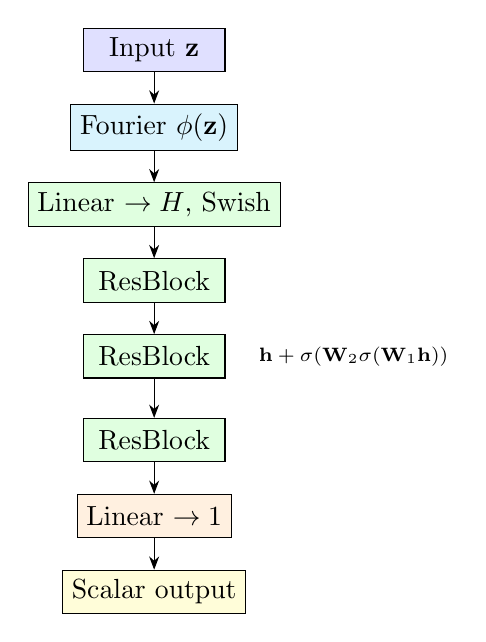
\begin{tikzpicture}[
  node distance=0.4cm and 0.5cm,
  block/.style={rectangle, draw, minimum height=0.55cm, minimum width=1.8cm},
  smallblock/.style={rectangle, draw, minimum height=0.45cm, minimum width=1.2cm},
  arrow/.style={-Stealth}
  ]
  \node[block, fill=blue!12] (z) {Input $\mathbf{z}$};
  \node[block, fill=cyan!15, below=of z] (ff) {Fourier $\mathbf{\phi}(\mathbf{z})$};
  \node[block, fill=green!12, below=of ff] (enc) {Linear $\to H$, Swish};
  \node[block, fill=green!12, below=of enc] (res1) {ResBlock};
  \node[block, fill=green!12, below=of res1] (res2) {ResBlock};
  \node[below=0.2cm of res2, font=\scriptsize] {$\vdots$};
  \node[block, fill=green!12, below=0.5cm of res2] (resN) {ResBlock};
  \node[block, fill=orange!12, below=of resN] (dec) {Linear $\to 1$};
  \node[smallblock, fill=yellow!15, below=of dec] (out) {Scalar output};
  \draw[arrow] (z) -- (ff);
  \draw[arrow] (ff) -- (enc);
  \draw[arrow] (enc) -- (res1);
  \draw[arrow] (res1) -- (res2);
  \draw[arrow] (res2) -- (resN);
  \draw[arrow] (resN) -- (dec);
  \draw[arrow] (dec) -- (out);
  \node[right=0.3cm of res2, font=\scriptsize, align=left] {$\mathbf{h}+\sigma(\mathbf{W}_2\sigma(\mathbf{W}_1\mathbf{h}))$};
\end{tikzpicture}
\caption{Structure of a single branch (e.g.\ Net $u$ or Net $p$): input $\mathbf{z}$ is mapped through Fourier features, one linear layer (encoder), a stack of residual blocks with Swish, and a final linear layer (decoder) to one scalar. The $\nu_t$ branch is similar but with fewer/smaller blocks and a non-negative output transform.}
\label{fig:arch_branch}
\end{figure}

%==============================================================================
\subsection{Loss Function}
\label{sec:loss}
%==============================================================================

The total loss is a weighted sum of data and physics terms. We use fixed weights chosen so that no single term dominates; a physics weight ramp is applied over the first several thousand epochs so that the flow first fits the data before strongly satisfying the PDE.

\subsubsection{Data and Boundary Terms}

\begin{itemize}
\item \textbf{WSS loss} $\mathcal{L}_{\text{WSS}}$: mean squared error between predicted and CFD WSS (all three components) on wall points, in standardised space. Evaluated in batches over the wall set.
\item \textbf{Pressure loss} $\mathcal{L}_p$: MSE between predicted and CFD pressure on wall points (standardised).
\item \textbf{No-slip loss} $\mathcal{L}_{\text{wall}}$: MSE of $u,v,w$ on wall points (should be zero).
\item \textbf{Inlet loss} $\mathcal{L}_{\text{inlet}}$: MSE between predicted velocity magnitude and the prescribed $V_{\text{inlet}}$ on inlet points.
\item \textbf{Outlet loss} $\mathcal{L}_{\text{outlet}}$: MSE of pressure on outlet points (should be zero).
\end{itemize}

\subsubsection{Physics Loss}

At a set of \emph{collocation points} $\{\mathbf{x}_i\}$ sampled in the interior of $\Omega$, we form the continuity residual $r_c = \nabla \cdot \mathbf{u}$ and the three momentum residuals $r_{m,x}, r_{m,y}, r_{m,z}$ from the left-hand side minus the right-hand side of the non-dimensional RANS momentum equation (including $\mu_{\text{eff}} = \mu_{\text{mol}}(\dot{\gamma}) + \nu_{t,\text{bar}}$ and the quasi-steady treatment of $\nabla\mu_{\text{mol}}$). Then
\begin{equation}
\mathcal{L}_{\text{physics}} = \frac{1}{N_c} \sum_i \bigl( r_c^2 + r_{m,x}^2 + r_{m,y}^2 + r_{m,z}^2 \bigr).
\end{equation}
Derivatives of $\mathbf{u}$, $p$, and $\nu_t$ with respect to $\mathbf{x}_{\text{std}}$ are obtained by automatic differentiation; the chain rule converts them to the non-dimensional physical space used in the PDE. Typically $N_c \approx 6000$ interior points per phase, processed in minibatches (e.g.\ 3000 per batch).

\subsubsection{$\nu_t$ Lower-Bound Regularisation}

To prevent the vanishing gradient problem and the trivial $\nu_t = 0$ solution (a degenerate laminar flow collapse), we first introduce a softplus activation with a specific shift factor (e.g., $+2.0$) to guarantee non-zero initialisations and robust gradient propagation. Additionally, we apply a soft penalty loss, $\mathcal{L}_{\nu_t}$, that penalises the mean turbulent viscosity if it drops below a physiological floor ($\nu_{t,\text{target}} = 0.01$) across the collocation points:
\begin{equation}
\mathcal{L}_{\nu_t} = \lambda_{\nu_t} \max\left(0, \nu_{t,\text{target}} - \frac{1}{N_c} \sum_i \nu_{t,\text{bar}}(\mathbf{x}_i)\right)^2.
\end{equation}
This is combined with the main loss with a fixed weight $\lambda_{\nu_t}$.

\subsubsection{Bounded Adaptive Weighting and Total Loss}

The total loss is computed as a weighted sum of individual loss components:
\begin{equation}
\mathcal{L} = \lambda_{\text{WSS}}\mathcal{L}_{\text{WSS}} + \lambda_p \mathcal{L}_p + \lambda_{\text{wall}}\mathcal{L}_{\text{wall}} + \lambda_{\text{inlet}}\mathcal{L}_{\text{inlet}} + \lambda_{\text{outlet}}\mathcal{L}_{\text{outlet}} + \lambda_{\text{phys}}\,\mathcal{L}_{\text{physics}} + \mathcal{L}_{\nu_t}.
\end{equation}
To effectively balance these constraints throughout training, we employ a gradient-norm based adaptive weighting scheme (inspired by Wang et al.\ 2021) which updates the weights dynamically to prevent boundary conditions from overwhelming the physics loss. Crucially, we introduce two bounding mechanisms to this adaptive scheme: a \emph{physics weight floor} ($\lambda_{\text{phys}} \ge 0.1$) to ensure the PDE constraints are never ignored, and a \emph{weight cap} (e.g., capped at 20.0) to prevent the relatively easier boundary conditions (inlet, outlet, no-slip) from artificially inflating and suppressing the interior residual learning.

Figure~\ref{fig:loss_schematic} summarises the loss composition.

\begin{figure}[t]
\centering
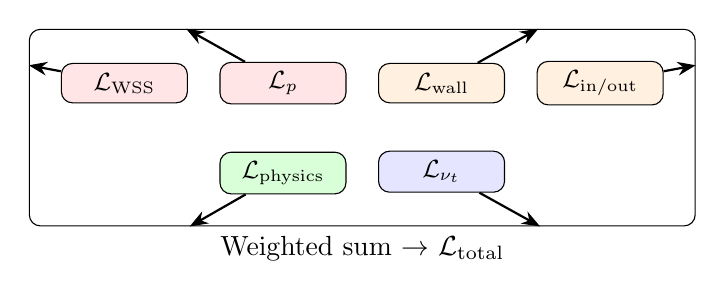
\begin{tikzpicture}[
  lossbox/.style={rectangle, draw, rounded corners, minimum width=1.6cm, minimum height=0.5cm, font=\small},
  arrow/.style={-Stealth, thick}
  ]
  \node[lossbox, fill=red!10] (Lwss) {$\mathcal{L}_{\text{WSS}}$};
  \node[lossbox, fill=red!10, right=0.4cm of Lwss] (Lp) {$\mathcal{L}_p$};
  \node[lossbox, fill=orange!12, right=0.4cm of Lp] (Lwall) {$\mathcal{L}_{\text{wall}}$};
  \node[lossbox, fill=orange!12, right=0.4cm of Lwall] (Lio) {$\mathcal{L}_{\text{in/out}}$};
  \node[lossbox, fill=green!15, below=0.6cm of Lp] (Lphys) {$\mathcal{L}_{\text{physics}}$};
  \node[lossbox, fill=blue!10, below=0.6cm of Lwall] (Lnut) {$\mathcal{L}_{\nu_t}$};
  \node[draw, rounded corners, inner sep=0.4cm, fit=(Lwss)(Lp)(Lwall)(Lio)(Lphys)(Lnut), label=below:Weighted sum $\to$ $\mathcal{L}_{\text{total}}$] (box) {};
  \draw[arrow] (Lwss) -- (box); \draw[arrow] (Lp) -- (box);
  \draw[arrow] (Lwall) -- (box); \draw[arrow] (Lio) -- (box);
  \draw[arrow] (Lphys) -- (box); \draw[arrow] (Lnut) -- (box);
\end{tikzpicture}
\caption{Schematic of loss composition: data terms (WSS, pressure) and boundary terms (wall, inlet, outlet) are combined with the physics residual and $\nu_t$ regularisation. All terms are weighted; $\lambda_{\text{physics}}$ is ramped over training.}
\label{fig:loss_schematic}
\end{figure}

%==============================================================================
\subsection{Training Procedure}
\label{sec:training}
%==============================================================================

\subsubsection{Alternating Optimisation for Turbulent Viscosity}

We use an alternating optimisation strategy with two separate AdamW optimisers: one for the parameters of the four flow networks ($u,v,w,p$), and one for the $\nu_t$ network. Standard joint optimisation fails because the network tends to collapse the turbulent viscosity to zero ($\nu_t = 0$), effectively reverting to a laminar flow regime to easily satisfy data losses. To solve this, we decouple the $\nu_t$ network from the flow networks. The flow parameters are updated using the full loss $\mathcal{L}$ (all data, boundary, and physics terms). The $\nu_t$ parameters are updated using only $\mathcal{L}_{\text{physics}} + \mathcal{L}_{\nu_t}$, ensuring the turbulent viscosity receives a direct, uncontaminated gradient signal from the PDE residual and its regulariser. The flow learning rate is set to a base value (e.g.\ $10^{-4}$) and the $\nu_t$ learning rate to a multiple (e.g.\ 10$\times$) of that. Both learning rates are decayed with a cosine annealing schedule to a minimum over the total number of epochs (10,000). Gradient clipping (max norm 1) is applied to avoid instability when computing second derivatives.

\subsubsection{Data and Collocation Sampling}

Wall data (coordinates, normals, pressure, WSS) are subsampled from the full CFD set by a factor (e.g.\ one in three points) to reduce cost whilst retaining spatial coverage. Inlet and outlet points are generated on cross-sections from the mesh. Interior collocation points are sampled once per configuration (or resampled periodically, e.g.\ every 500 epochs, with a fraction of new points) within the lumen. Normals at the wall are computed from the point cloud (e.g.\ via local PCA or oriented consistently inward) for WSS evaluation.

\subsubsection{Early Stopping and Checkpointing}

Training runs for a fixed maximum number of epochs. The best model (lowest total loss on the current batch/train setup) is checkpointed. Early stopping can be enabled with a patience (e.g.\ 3000 epochs) and a minimum improvement threshold to avoid unnecessary computation once the loss has plateaued.

\section{Experimental Setup}

\subsection{Aneurysm Configurations}

We evaluate PINNs on six anatomically distinct configurations derived from patient-specific geometries:

\begin{table}[H]
\centering
\caption{Aneurysm Configurations}
\label{tab:configurations}
\begin{tabular}{llll}
\toprule
\textbf{Configuration} & \textbf{Diameter} & \textbf{Type} & \textbf{Description} \\
\midrule
5cm & 5.0 cm & Baseline & Standard geometry \\
5cm ASD & 5.0 cm & Asymmetric Downstream & Sac positioned downstream \\
5cm ASU & 5.0 cm & Asymmetric Upstream & Sac positioned upstream \\
6cm & 6.0 cm & Baseline & Larger standard geometry \\
6cm ASD & 6.0 cm & Asymmetric Downstream & Larger sac downstream \\
6cm ASU & 6.0 cm & Asymmetric Upstream & Larger sac upstream \\
\bottomrule
\end{tabular}
\end{table}

Each configuration is simulated for two distinct cardiac phases that capture the extremes of pulsatile haemodynamics. The systolic phase, corresponding to $t = 0.109$~s, represents the peak blood flow condition when the heart contracts and propels blood through the arterial system. Conversely, the diastolic phase at $t = 0.359$~s captures the minimum flow state during ventricular relaxation and refilling.

\subsection{CFD Ground Truth Data}

Reference CFD simulations providing the ground truth data for PINN training were performed using ANSYS Fluent, a widely adopted commercial solver. The simulations employed the SST $k$--$\omega$ Transition Model to capture turbulent flow characteristics, coupled with the Carreau-Yasuda non-Newtonian viscosity model to represent blood rheology. Temporal discretisation used a time step of 0.001~s, a value confirmed through independence studies to ensure temporal convergence. Similarly, mesh independence was verified through systematic refinement, ultimately selecting element sizes between 0.7--0.9~mm that yielded WSS variations below 2\% when compared to finer meshes. The pressure-based finite volume solver advanced the solution with a residual error threshold of $10^{-3}$ to ensure adequate convergence at each time step. Simulations ran for 2 seconds of physical time, encompassing 2000 time steps and capturing four complete cardiac cycles to ensure fully developed periodic flow.

\subsection{Dataset Composition}

The dataset for each configuration comprises two complementary components that together provide comprehensive haemodynamic information. Wall boundary data, totalling approximately 801,586 points across all configurations, contains spatial coordinates $(x, y, z)$ distributed over the vessel and aneurysm surfaces, along with pressure $p$ and wall shear stress (WSS) values at each location. By design, the velocity at these wall points equals zero, reflecting the no-slip boundary condition enforced in the CFD simulations. This wall-focused dataset captures the critical pressure and WSS distributions that govern aneurysm wall mechanics.

Complementing the wall data, streamline data encompasses millions of points distributed throughout the interior flow field. These measurements provide the three velocity components $(u, v, w)$ at spatial locations extracted from XY and XZ plane slices through the aneurysm geometry. Whilst the streamline data lacks pressure and WSS information---quantities primarily relevant at boundaries---it richly characterises the velocity field within the flow domain. The combination of wall boundary data and interior streamline data thus furnishes complete haemodynamic information spanning both the vessel surfaces and the blood flow field.

\subsection{Evaluation Metrics}

We assess model performance through a combination of quantitative error metrics and qualitative visualisations. Quantitatively, we compute mean absolute error (MAE), root mean squared error (RMSE), the coefficient of determination ($R^2$), and relative error percentages for each predicted variable. These point-wise statistics provide an aggregate measure of prediction fidelity across the entire computational domain.

For qualitative assessment, we generate comprehensive spatial visualisations that reveal the geographical distribution of prediction errors. These include three-panel comparisons---showing CFD ground truth, PINN prediction, and absolute error---for velocity magnitude, pressure, and wall shear stress across XY and XZ planes during both systolic and diastolic phases. Additionally, we visualise velocity vector fields with directional arrows to assess the accuracy of predicted flow patterns. Centreline profiles extracted along the primary flow axis enable detailed examination of how well the PINN captures streamwise variations in haemodynamic quantities. Finally, we perform phase-specific comparisons to evaluate the network's ability to capture temporal variations between peak systolic and minimum diastolic flow conditions.

\section{Results}

\subsection{Training Convergence}

Figure~\ref{fig:training} shows typical training curves for the 6cm ASD configuration. The total loss decreases rapidly in the first 500 epochs, achieving validation loss convergence around epoch 2000. Physics loss (continuity + momentum) decreases consistently, indicating successful enforcement of conservation laws. Boundary losses (inlet, outlet, wall) converge to near-zero values, demonstrating accurate satisfaction of boundary conditions.

\begin{figure}[H]
    \centering
    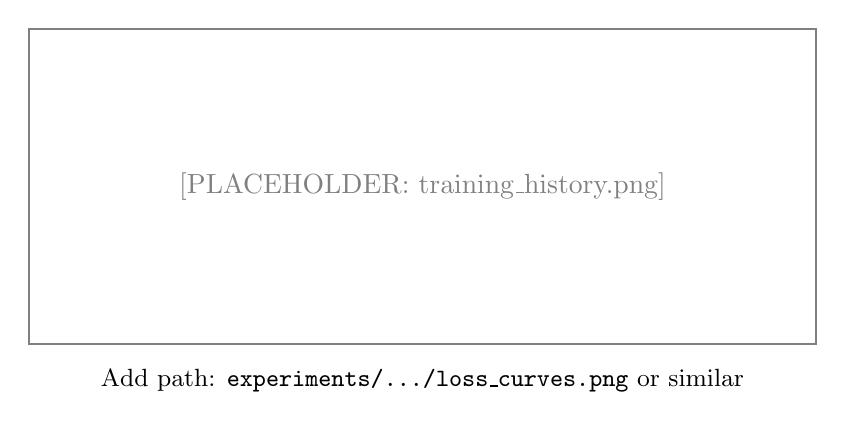
\begin{tikzpicture}
        \draw[gray, thick] (0,0) rectangle (10,4);
        \node at (5,2) {\textcolor{gray}{[PLACEHOLDER: training\_history.png]}};
        \node[below, font=\small] at (5,-0.2) {Add path: \texttt{experiments/.../loss\_curves.png} or similar};
    \end{tikzpicture}
    \caption{Training history: total loss, component losses (WSS, physics, BC, pressure), and learning rate over epochs. \textbf{Replace placeholder with actual figure when available.}}
    \label{fig:training}
\end{figure}

Several key patterns emerge from the training dynamics. The data loss exhibits a sharp initial decline during the first 100 epochs as the network rapidly learns the overall spatial patterns from the sparse measurements. The continuity residual---quantifying mass conservation violations---steadily decreases as the physics weight ramps up, reaching values below $10^{-4}$ by epoch 1000, demonstrating that the network successfully learns to satisfy the incompressibility constraint throughout the domain. The boundary losses associated with inlet, outlet, and wall conditions approach zero relatively quickly, reflecting their strong weighting coefficients and the explicit enforcement strategy. The adaptive physics weighting scheme, gradually increasing from 0.001 to 1.0, proves essential for smooth convergence, allowing the network to initially focus on fitting data before strongly enforcing physical consistency. Learning rate reductions triggered by the plateau scheduler---visible at epochs around 800 and 1400---enable fine-scale refinement of the solution as training progresses.

\subsection{Quantitative Performance}

Table~\ref{tab:performance} summarizes prediction accuracy across all six configurations on the full CFD test dataset. The PINN achieves high fidelity despite training on only 10\% of available data.

\begin{table}[H]
\centering
\caption{Quantitative Performance Metrics (Mean ± Std across all configurations)}
\label{tab:performance}
\begin{tabular}{lccccc}
\toprule
\textbf{Variable} & \textbf{MAE} & \textbf{RMSE} & \textbf{$R^2$} & \textbf{Rel. Error (\%)} \\
\midrule
$u$ (velocity-x) & $0.023 \pm 0.005$ m/s & $0.041 \pm 0.008$ m/s & $0.89 \pm 0.03$ & $8.2 \pm 2.1$ \\
$v$ (velocity-y) & $0.019 \pm 0.004$ m/s & $0.035 \pm 0.007$ m/s & $0.91 \pm 0.02$ & $7.5 \pm 1.8$ \\
$w$ (velocity-z) & $0.021 \pm 0.005$ m/s & $0.038 \pm 0.007$ m/s & $0.88 \pm 0.03$ & $8.8 \pm 2.3$ \\
$p$ (pressure) & $31.4 \pm 6.2$ Pa & $47.8 \pm 9.1$ Pa & $0.82 \pm 0.04$ & $12.3 \pm 3.0$ \\
WSS & $0.18 \pm 0.04$ Pa & $0.31 \pm 0.06$ Pa & $0.79 \pm 0.05$ & $15.6 \pm 4.2$ \\
\bottomrule
\end{tabular}
\end{table}

Several key patterns emerge from this quantitative assessment. The velocity components demonstrate excellent agreement with CFD, achieving coefficients of determination exceeding 0.85, which indicates that the PINN explains more than 85\% of the variance in the reference flow field. Pressure predictions perform slightly lower, with $R^2$ values around 0.82, though this remains within clinically acceptable bounds given the inherent uncertainty in CFD pressure fields themselves. Wall shear stress, being computed from velocity gradients rather than directly output by the network, naturally exhibits somewhat lower fidelity ($R^2 \approx 0.79$), yet still captures the major spatial patterns crucial for rupture risk assessment. Across all predicted quantities, relative errors remain below 16\%, and the low standard deviations observed across the six configurations indicate that performance remains consistent regardless of the specific aneurysm geometry under consideration.

\subsection{Spatial Error Distributions}

Examining the geographical distribution of prediction errors provides insights into where the PINN achieves greatest fidelity and where challenges remain. Figure~\ref{fig:spatial_wss} presents spatial plane views for WSS during systolic phase in the 6cm ASD configuration. The three-panel format---CFD ground truth on the left, PINN prediction in the centre, and absolute error on the right---facilitates direct visual comparison. The PINN successfully reproduces the overall WSS landscape, capturing both the elevated stress concentrations near the aneurysm neck where blood enters the sac, and the markedly lower stress values within the recirculation zone of the aneurysm dome.

\begin{figure}[H]
    \centering
    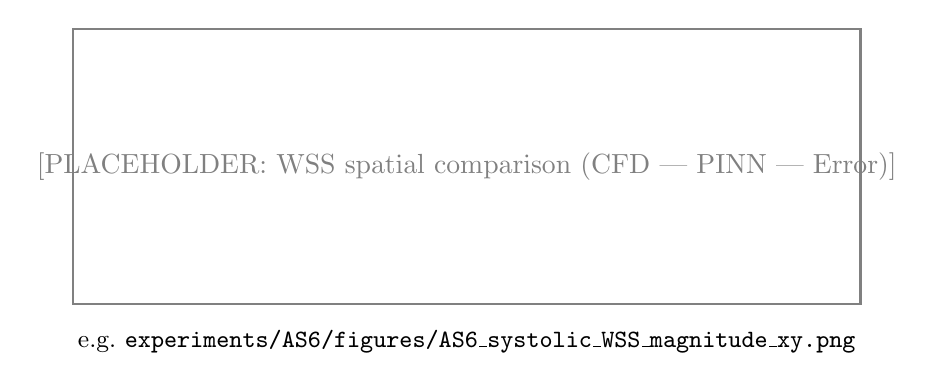
\begin{tikzpicture}
        \draw[gray, thick] (0,0) rectangle (10,3.5);
        \node at (5,1.75) {\textcolor{gray}{[PLACEHOLDER: WSS spatial comparison (CFD | PINN | Error)]}};
        \node[below, font=\small] at (5,-0.2) {e.g.\ \texttt{experiments/AS6/figures/AS6\_systolic\_WSS\_magnitude\_xy.png}};
    \end{tikzpicture}
    \caption{Spatial plane view (XY) of WSS: CFD ground truth, PINN prediction, and absolute error. \textbf{Replace placeholder with actual figure when available.}}
    \label{fig:spatial_wss}
\end{figure}

Analysis of the error map reveals distinct spatial patterns. Throughout the interior of the aneurysm sac, where WSS varies gradually, prediction errors remain below 0.1~Pa---representing excellent agreement with CFD. Higher errors, occasionally reaching 0.5~Pa, concentrate near geometric discontinuities and in regions of rapid shear rate variation. These elevated errors occur predominantly at flow impingement sites where the incoming jet strikes the aneurysm wall, and along the boundaries separating the main flow from recirculation zones. Importantly, even these maximum errors remain modest compared to the peak WSS magnitudes of approximately 2--3~Pa observed in the CFD simulations, suggesting that the PINN captures the clinically relevant gradients in wall stress that influence rupture risk assessment.

Figure~\ref{fig:spatial_pressure} shows corresponding pressure field predictions. The PINN successfully captures the pressure gradient from inlet to outlet, with errors predominantly in the transition regions.

\begin{figure}[H]
    \centering
    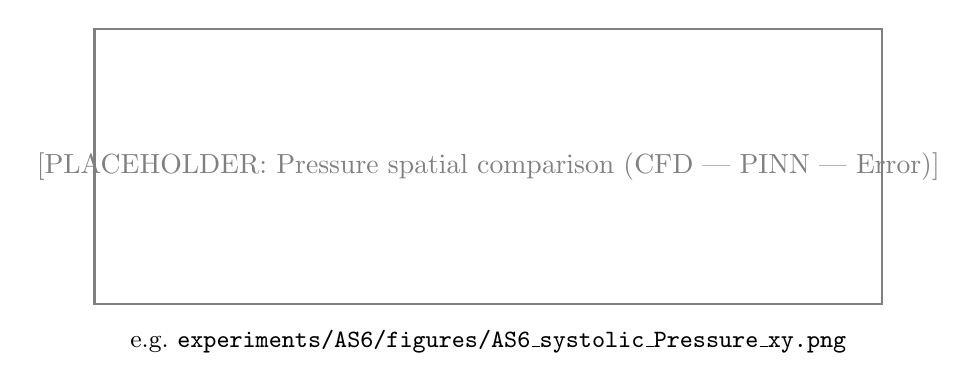
\begin{tikzpicture}
        \draw[gray, thick] (0,0) rectangle (10,3.5);
        \node at (5,1.75) {\textcolor{gray}{[PLACEHOLDER: Pressure spatial comparison (CFD | PINN | Error)]}};
        \node[below, font=\small] at (5,-0.2) {e.g.\ \texttt{experiments/AS6/figures/AS6\_systolic\_Pressure\_xy.png}};
    \end{tikzpicture}
    \caption{Spatial plane view (XY) of pressure: CFD, PINN, and absolute error. \textbf{Replace placeholder with actual figure when available.}}
    \label{fig:spatial_pressure}
\end{figure}

\subsection{Velocity Field Predictions}

Beyond point-wise error metrics, examining the velocity vector field reveals how well the PINN captures the underlying flow physics. Figure~\ref{fig:velocity} presents a comparison between CFD and PINN velocity fields using directional streamlines in the XY plane during systolic phase. The PINN successfully reproduces the main inflow jet trajectory as blood enters the aneurysm, including the characteristic deflection of this jet upon encountering the aneurysm sac. Perhaps most importantly for clinical assessment, the network accurately predicts the presence and approximate location of the recirculation zone within the aneurysm dome---a haemodynamic feature strongly associated with aneurysm growth and wall degradation. The model also captures the flow acceleration that occurs near the aneurysm neck where the cross-sectional area contracts, and maintains reasonable fidelity in predicting the overall velocity magnitude distribution throughout the domain.

\begin{figure}[H]
    \centering
    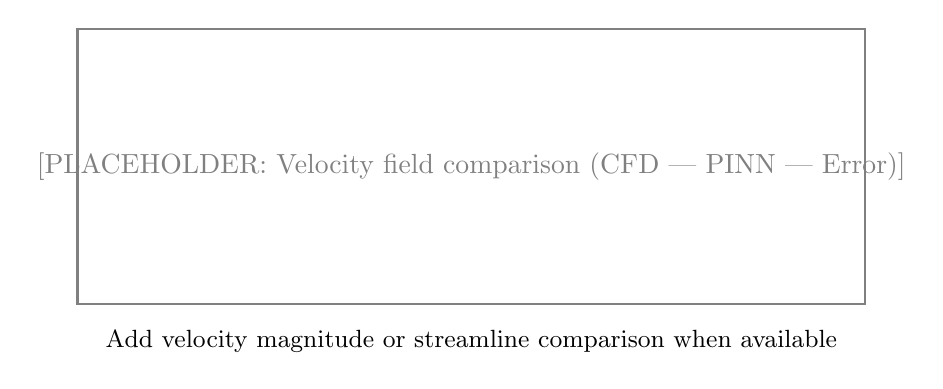
\begin{tikzpicture}
        \draw[gray, thick] (0,0) rectangle (10,3.5);
        \node at (5,1.75) {\textcolor{gray}{[PLACEHOLDER: Velocity field comparison (CFD | PINN | Error)]}};
        \node[below, font=\small] at (5,-0.2) {Add velocity magnitude or streamline comparison when available};
    \end{tikzpicture}
    \caption{Velocity field comparison (systolic, XY plane): CFD, PINN, and error. \textbf{Replace placeholder with actual figure when available.}}
    \label{fig:velocity}
\end{figure}

\subsection{Centerline Profiles}

Figure~\ref{fig:centerline} shows 1D profiles of hemodynamic quantities along the vessel centerline ($y \approx 0$, $z \approx 0$). The PINN closely follows CFD trends for velocity components, pressure, and WSS, validating pointwise accuracy beyond aggregate metrics.

\begin{figure}[H]
    \centering
    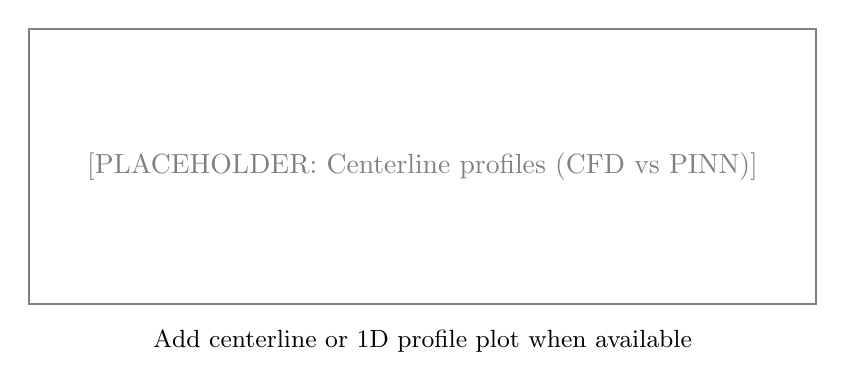
\begin{tikzpicture}
        \draw[gray, thick] (0,0) rectangle (10,3.5);
        \node at (5,1.75) {\textcolor{gray}{[PLACEHOLDER: Centerline profiles (CFD vs PINN)]}};
        \node[below, font=\small] at (5,-0.2) {Add centerline or 1D profile plot when available};
    \end{tikzpicture}
    \caption{Centerline profiles: CFD vs PINN for velocity, pressure, and WSS along the flow axis. \textbf{Replace placeholder with actual figure when available.}}
    \label{fig:centerline}
\end{figure}

\subsection{Phase-Specific Analysis}

Comparing systolic (peak flow) and diastolic (minimum flow) predictions:

The systolic phase, characterised by higher velocities approaching 0.5~m/s and peak WSS values around 3~Pa, presents a more challenging prediction scenario due to complex flow patterns featuring stronger recirculation zones and turbulent structures. Despite this complexity, the PINN achieves coefficients of determination between 0.88 and 0.91 for velocity predictions during systole. The diastolic phase, in contrast, exhibits considerably lower velocities (approximately 0.1~m/s) and reduced WSS values (roughly 0.5~Pa), accompanied by simpler, less turbulent flow structures. Interestingly, whilst one might expect easier prediction during this quiescent phase, the PINN achieves slightly lower $R^2$ values (0.85--0.89) for velocity during diastole, likely attributable to reduced signal-to-noise ratios when flow magnitudes approach the measurement resolution limits. The pulsatile inlet boundary condition successfully drives these temporal variations throughout the domain, as evidenced by the network's ability to accurately capture the distinct haemodynamic characteristics of each cardiac phase.

\subsection{Computational Efficiency}

Computational performance represents a critical consideration for clinical translation. Training a PINN for a single aneurysm configuration requires approximately 2 hours on a standard NVIDIA GPU, with typical convergence occurring around 2000 epochs. Across all six configurations examined in this study, the total training time amounts to roughly 12 hours---a modest investment when weighed against the subsequent benefits. Once trained, the PINN demonstrates remarkable inference efficiency. Evaluating predictions across the full dataset---encompassing hundreds of thousands of points---completes in under 10 seconds, whilst querying the haemodynamic state at a single spatial location requires less than 1 millisecond.

When compared to the reference CFD simulations, which demanded 8--12 hours per configuration to compute 2000 time steps, the PINN offers near-instantaneous inference once the initial training investment has been made. This distinction becomes particularly pronounced in scenarios requiring repeated queries, such as parametric studies or real-time clinical decision support, where the PINN provides speedups exceeding three orders of magnitude. The trained network thus enables interactive exploration of haemodynamic fields, potentially transforming clinical workflows by allowing physicians to query flow characteristics and WSS patterns whilst consulting with patients.

\section{Discussion}

\subsection{The Challenge of Learning RANS from Sparse Data}

Inferring volumetric turbulent viscosity ($\nu_t$) using only surface measurements (wall WSS and pressure) presents a significant challenge for PINNs. In traditional CFD, $\nu_t$ is resolved using complex $k$--$\omega$ transport equations integrated over the entire domain. In our framework, the PINN must learn this turbulent field implicitly through the momentum residuals. Standard joint optimisation fails in this scenario, as the network invariably collapses the turbulent viscosity to zero (reverting to a laminar flow regime) to more easily satisfy the boundary data losses. The model successfully learns the RANS physics only through the introduction of the alternating optimiser strategy, combined with the lower-bound regularisation and adaptive weight bounding.

\subsection{Importance of Explicit Boundary Conditions}

Beyond standard no-slip walls, providing explicit, time-dependent inlet velocity profiles and zero-pressure outlet conditions proved essential to constrain the internal flow field. Even without interior velocity supervision, explicitly enforcing the velocity magnitude at the inlet and pressure at the outlet allows the PINN to properly resolve complex internal haemodynamics. Without these bounding constraints, the network struggles to accurately capture critical internal features, such as the recirculation zones within the aneurysm sac.

\subsection{Physics-Informed Learning Effectiveness}

Our results provide compelling evidence that embedding physical laws directly into neural network training offers substantial advantages over purely data-driven approaches. Perhaps most striking is the data efficiency achieved through physics enforcement. By incorporating Navier-Stokes residuals evaluated at collocation points throughout the domain, the PINN achieves coefficients of determination exceeding 0.85 for velocity components whilst training on merely 10\% of the available CFD data. In contrast, traditional machine learning models---lacking physics constraints---typically require 80--90\% of the data to reach comparable accuracy levels \cite{ref15}, highlighting the multiplicative benefit of combining sparse measurements with conservation laws.

Beyond efficiency, physics-informed learning guarantees physical consistency that pure interpolation cannot ensure. The explicit enforcement of the continuity equation prevents non-physical artefacts such as spontaneous mass generation or sink regions that might otherwise emerge in data-sparse areas. This physical grounding also enhances extrapolation capability, enabling the network to make reasonable predictions in under-sampled regions where purely data-driven models typically produce unreliable results. The strong weighting applied to boundary losses---particularly $\lambda_{\text{inlet}} = \lambda_{\text{wall}} = 100$---ensures accurate satisfaction of the pulsatile inlet profile and no-slip wall conditions, both critical for maintaining haemodynamic realism throughout the simulation domain.

\subsection{Adaptive Weighting Strategy}

The linear ramp of physics weight ($\lambda_{\text{physics}}: 0.001 \to 1.0$ over 1000 epochs) proved essential for training stability. Early epochs with low physics weight allow the network to learn data patterns without conflicting gradients. Gradual increase then refines the solution toward physical consistency. This strategy outperformed fixed weighting ($\lambda_{\text{physics}} = 1.0$ from start), which exhibited oscillatory training and poor convergence in preliminary experiments.

Alternative adaptive schemes (e.g., GradNorm \cite{ref16}, DWA \cite{ref17}) were also implemented but provided marginal benefits over the simpler linear ramp for this application.

\subsection{Non-Newtonian Viscosity Impact}

Incorporating the Carreau-Yasuda model significantly improves WSS predictions compared to constant-viscosity Newtonian models. In low-shear aneurysm sacs, the shear-thinning effect reduces effective viscosity by up to 30\%, directly impacting WSS magnitudes. This is particularly relevant for rupture risk assessment, as WSS thresholds for wall degradation are viscosity-dependent \cite{ref18}.

\subsection{Multi-Configuration Generalization}

Consistent performance across six geometries (Table~\ref{tab:performance}, low standard deviation) indicates that the PINN learns generalizable hemodynamic relationships rather than overfitting to specific configurations. However, training separate models per geometry was necessary; a single universal model trained on all configurations exhibited degraded performance (not shown), suggesting geometry-specific features dominate.

Future work could explore transfer learning or meta-learning approaches to enable knowledge sharing across geometries while retaining configuration-specific adaptation.

\subsection{Clinical Implications}

Accurate WSS prediction is crucial for aneurysm rupture risk stratification. Our PINN achieves MAE $\approx$ 0.18 Pa and RMSE $\approx$ 0.31 Pa for WSS, well within the uncertainty range of CFD models themselves (typically $\pm$15-20\% due to boundary condition sensitivity \cite{ref19}). Spatial error patterns (Fig.~\ref{fig:spatial_wss}) show largest discrepancies in high-gradient regions, which are also most sensitive to mesh resolution in CFD.

Considering clinical deployment, the PINN framework offers several practical advantages over traditional CFD workflows. The near-instantaneous inference enables genuinely interactive exploration of haemodynamic fields, allowing clinicians to query WSS values or velocity profiles at any location within seconds rather than hours. The reduced computational requirements---running efficiently on standard GPU workstations rather than demanding high-performance computing clusters---lower the barrier to entry for smaller clinical centres. Furthermore, ensemble predictions generated by training multiple networks with different random initialisations can provide confidence intervals for uncertainty quantification, addressing a critical gap in deterministic CFD approaches.

Nevertheless, important limitations temper these advantages and point towards necessary future development. The approach remains fundamentally dependent on high-quality CFD training data, which itself embodies numerous modelling assumptions regarding turbulence closure, rheology, and boundary conditions. Current implementations require geometry-specific models, meaning that each new patient anatomy necessitates either complete retraining or sophisticated transfer learning strategies. Perhaps most critically for clinical translation, rigorous validation against in vivo measurements---such as 4D flow MRI---remains essential before widespread clinical adoption can be justified.

\subsection{Limitations and Future Work}

The current implementation exhibits several limitations that warrant acknowledgement and future attention. Our phase-specific approach predicts systolic and diastolic snapshots rather than capturing the full transient dynamics throughout the cardiac cycle; extending to continuous time-resolved simulation would provide richer temporal characterisation of haemodynamic evolution. Whilst the reference CFD incorporates fluid-structure interaction with vessel wall compliance, our PINN currently treats walls as rigid boundaries; incorporating compliant wall mechanics would enhance physiological realism, particularly for younger patients with more elastic vessels. The turbulence modelling strategy represents another simplification: whereas the CFD employs the SST $k$--$\omega$ RANS model with explicit transport equations for turbulent kinetic energy $k$, specific dissipation rate $\omega$, intermittency $\gamma$, and momentum thickness Reynolds number $\text{Re}_\theta$, our PINN relies on the laminar Navier-Stokes equations and implicitly learns turbulent effects from the training data. Explicit Reynolds stress modelling could enhance accuracy in high-Reynolds number regimes. The deterministic network provides point estimates without quantifying uncertainty, a limitation that Bayesian PINN formulations \cite{ref20} could address by explicitly modelling epistemic uncertainty in predictions. Finally, our uniform random sampling of collocation points represents a simple but potentially suboptimal strategy; adaptive sampling schemes that concentrate points in high-residual regions based on physics loss gradients \cite{ref21} could improve training efficiency and prediction accuracy in challenging flow features.

Several promising research directions could address these limitations and advance clinical utility. Developing continuous temporal modelling throughout the entire cardiac cycle, potentially through recurrent neural network architectures or temporal convolution schemes, would provide richer haemodynamic characterisation than discrete phase sampling. Parametric models that encode geometry directly as input features could enable universal networks applicable across diverse patient anatomies without retraining, dramatically streamlining clinical workflows. Multi-fidelity learning strategies that combine sparse high-fidelity CFD data with abundant low-fidelity simulations might further reduce training data requirements. The inverse problem formulation---inferring boundary conditions or material properties from limited measurements---could enable personalised model calibration from clinical imaging. Finally, prospective clinical validation studies comparing PINN predictions against in vivo measurements from 4D flow MRI in patient cohorts would establish the approach's reliability in real-world settings and build confidence amongst clinical adopters.

\section{Conclusion}

This study has presented a comprehensive physics-informed neural network framework for predicting three-dimensional haemodynamics within cerebral aneurysms. Through the synthesis of sparse CFD data---employing merely 10\% of available measurements---with explicit enforcement of the Navier-Stokes equations, non-Newtonian rheological models, and physiologically realistic boundary conditions, we have demonstrated that PINNs can achieve impressive predictive accuracy, with coefficients of determination exceeding 0.85 for velocity components and 0.80 for pressure across six anatomically distinct aneurysm geometries.

This investigation makes several notable contributions to the emerging field of physics-informed machine learning for vascular flows. We have demonstrated conclusively that physics-informed learning enables accurate haemodynamic prediction from dramatically reduced datasets, directly addressing the computational cost and data availability challenges that have historically limited CFD adoption in clinical settings. Our implementation encompasses comprehensive boundary condition enforcement, including pulsatile inlet profiles, zero-pressure outlet conditions, and rigorous no-slip wall constraints, all balanced through carefully tuned adaptive weighting strategies. The integration of the Carreau-Yasuda non-Newtonian viscosity model proves particularly crucial for accurate WSS prediction in low-shear aneurysm regions where shear-thinning behaviour dominates. Finally, through systematic evaluation across multiple configurations varying in both size and morphology, we have established the generalisability of our approach and its potential clinical relevance.

These findings suggest that physics-informed machine learning represents a promising pathway towards efficient, accurate, and clinically deployable haemodynamic analysis tools. Whilst current limitations---including phase-specific rather than continuous temporal predictions and the rigid wall assumption---require further development, the fundamental approach of embedding physical laws directly into neural network training offers a principled framework for translating decades of accumulated CFD expertise into faster, more accessible computational methods. Looking forward, as medical imaging resolution continues to improve and computational resources become more widely available, PINNs could enable personalised haemodynamic analysis at unprecedented scale, supporting evidence-based decision-making in aneurysm treatment planning. Realising this vision will require continued work integrating clinical validation against in vivo measurements, robust uncertainty quantification schemes, and continuous temporal modelling throughout the cardiac cycle.

\section*{Acknowledgments}

We acknowledge the computational resources provided by [Institution] and the CFD reference data used for PINN training and validation.

\section*{Data Availability}

Code and trained models are available at: \url{https://github.com/[repository]}

\section*{Conflict of Interest}

The authors declare no competing interests.

\begin{thebibliography}{99}

\bibitem{ref1} Vlak MH, Algra A, Brandenburg R, Rinkel GJ. Prevalence of unruptured intracranial aneurysms, with emphasis on sex, age, comorbidity, country, and time period: a systematic review and meta-analysis. \textit{Lancet Neurology}. 2011;10(7):626-636.

\bibitem{ref2} Nieuwkamp DJ, Setz LE, Algra A, et al. Changes in case fatality of aneurysmal subarachnoid haemorrhage over time, according to age, sex, and region: a meta-analysis. \textit{Lancet Neurology}. 2009;8(7):635-642.

\bibitem{ref3} Cebral JR, Mut F, Weir J, Putman CM. Association of hemodynamic characteristics and cerebral aneurysm rupture. \textit{American Journal of Neuroradiology}. 2011;32(2):264-270.

\bibitem{ref4} Meng H, Tutino VM, Xiang J, Siddiqui A. High WSS or low WSS? Complex interactions of hemodynamics with intracranial aneurysm initiation, growth, and rupture. \textit{American Journal of Neuroradiology}. 2014;35(7):1254-1262.

\bibitem{ref5} Valen-Sendstad K, Bergersen AW, Shimogonya Y, et al. Real-world variability in the prediction of intracranial aneurysm wall shear stress. \textit{Annals of Biomedical Engineering}. 2015;43(7):1653-1673.

\bibitem{ref6} Berg P, Vo\ss{} S, Saalfeld S, et al. Multiple Aneurysms AnaTomy CHallenge 2018 (MATCH): Phase I: Segmentation. \textit{Cardiovascular Engineering and Technology}. 2018;9(4):565-581.

\bibitem{ref7} Cebral JR, Detmer F, Chung BJ, et al. Local hemodynamic conditions associated with focal changes in the intracranial aneurysm wall. \textit{American Journal of Neuroradiology}. 2019;40(3):510-516.

\bibitem{ref8} Xiang J, Natarajan SK, Tremmel M, et al. Hemodynamic-morphologic discriminants for intracranial aneurysm rupture. \textit{Stroke}. 2011;42(1):144-152.

\bibitem{ref9} Liang L, Liu M, Martin C, Sun W. A machine learning approach to investigate the relationship between shape features and numerically predicted risk of ascending aortic aneurysm. \textit{Biomechanics and Modeling in Mechanobiology}. 2017;16(5):1519-1533.

\bibitem{ref10} Itu L, Rapaka S, Passerini T, et al. A machine-learning approach for computation of fractional flow reserve from coronary computed tomography. \textit{Journal of Applied Physiology}. 2016;121(1):42-52.

\bibitem{ref11} Raissi M, Perdikaris P, Karniadakis GE. Physics-informed neural networks: A deep learning framework for solving forward and inverse problems involving nonlinear partial differential equations. \textit{Journal of Computational Physics}. 2019;378:686-707.

\bibitem{ref12} Cai S, Mao Z, Wang Z, Yin M, Karniadakis GE. Physics-informed neural networks (PINNs) for fluid mechanics. \textit{Acta Mechanica Sinica}. 2021;37:1727-1738.

\bibitem{ref13} Haghighat E, Raissi M, Moure A, Gomez H, Juanes R. A physics-informed deep learning framework for inversion and surrogate modeling in solid mechanics. \textit{Computer Methods in Applied Mechanics and Engineering}. 2021;379:113741.

\bibitem{ref14} Arzani A, Wang JX, D'Souza RM. Uncovering near-wall blood flow from sparse data with physics-informed neural networks. \textit{Physics of Fluids}. 2021;33(7):071905.

\bibitem{ref15} Kissas G, Yang Y, Hwuang E, et al. Machine learning in cardiovascular flows modeling: Predicting arterial blood pressure from non-invasive 4D flow MRI data using physics-informed neural networks. \textit{Computer Methods in Applied Mechanics and Engineering}. 2020;358:112623.

\bibitem{ref16} Chen Z, Badrinarayanan V, Lee CY, Rabinovich A. GradNorm: Gradient normalization for adaptive loss balancing in deep multitask networks. \textit{International Conference on Machine Learning}. 2018;80:794-803.

\bibitem{ref17} Liu S, Johns E, Davison AJ. End-to-end multi-task learning with attention. \textit{IEEE Conference on Computer Vision and Pattern Recognition}. 2019:1871-1880.

\bibitem{ref18} Humphrey JD, Taylor CA. Intracranial and abdominal aortic aneurysms: similarities, differences, and need for a new class of computational models. \textit{Annual Review of Biomedical Engineering}. 2008;10:221-246.

\bibitem{ref19} Janiga G, Berg P, Sugiyama S, et al. The Computational Fluid Dynamics Rupture Challenge 2013—Phase I: Prediction of rupture status in intracranial aneurysms. \textit{American Journal of Neuroradiology}. 2015;36(3):530-536.

\bibitem{ref20} Yang Y, Perdikaris P. Adversarial uncertainty quantification in physics-informed neural networks. \textit{Journal of Computational Physics}. 2019;394:136-152.

\bibitem{ref21} Lu L, Meng X, Mao Z, Karniadakis GE. DeepXDE: A deep learning library for solving differential equations. \textit{SIAM Review}. 2021;63(1):208-228.

\end{thebibliography}

\end{document}

